% Options for packages loaded elsewhere
\PassOptionsToPackage{unicode}{hyperref}
\PassOptionsToPackage{hyphens}{url}
%
\documentclass[
]{article}
\usepackage{amsmath,amssymb}
\usepackage{lmodern}
\usepackage{iftex}
\ifPDFTeX
  \usepackage[T1]{fontenc}
  \usepackage[utf8]{inputenc}
  \usepackage{textcomp} % provide euro and other symbols
\else % if luatex or xetex
  \usepackage{unicode-math}
  \defaultfontfeatures{Scale=MatchLowercase}
  \defaultfontfeatures[\rmfamily]{Ligatures=TeX,Scale=1}
\fi
% Use upquote if available, for straight quotes in verbatim environments
\IfFileExists{upquote.sty}{\usepackage{upquote}}{}
\IfFileExists{microtype.sty}{% use microtype if available
  \usepackage[]{microtype}
  \UseMicrotypeSet[protrusion]{basicmath} % disable protrusion for tt fonts
}{}
\makeatletter
\@ifundefined{KOMAClassName}{% if non-KOMA class
  \IfFileExists{parskip.sty}{%
    \usepackage{parskip}
  }{% else
    \setlength{\parindent}{0pt}
    \setlength{\parskip}{6pt plus 2pt minus 1pt}}
}{% if KOMA class
  \KOMAoptions{parskip=half}}
\makeatother
\usepackage{xcolor}
\usepackage[margin=1in]{geometry}
\usepackage{graphicx}
\makeatletter
\def\maxwidth{\ifdim\Gin@nat@width>\linewidth\linewidth\else\Gin@nat@width\fi}
\def\maxheight{\ifdim\Gin@nat@height>\textheight\textheight\else\Gin@nat@height\fi}
\makeatother
% Scale images if necessary, so that they will not overflow the page
% margins by default, and it is still possible to overwrite the defaults
% using explicit options in \includegraphics[width, height, ...]{}
\setkeys{Gin}{width=\maxwidth,height=\maxheight,keepaspectratio}
% Set default figure placement to htbp
\makeatletter
\def\fps@figure{htbp}
\makeatother
\setlength{\emergencystretch}{3em} % prevent overfull lines
\providecommand{\tightlist}{%
  \setlength{\itemsep}{0pt}\setlength{\parskip}{0pt}}
\setcounter{secnumdepth}{-\maxdimen} % remove section numbering
\ifLuaTeX
  \usepackage{selnolig}  % disable illegal ligatures
\fi
\IfFileExists{bookmark.sty}{\usepackage{bookmark}}{\usepackage{hyperref}}
\IfFileExists{xurl.sty}{\usepackage{xurl}}{} % add URL line breaks if available
\urlstyle{same} % disable monospaced font for URLs
\hypersetup{
  pdftitle={2013 CSMI Zooplankton Stable Isotope Data Exploration},
  pdfauthor={Kayden},
  hidelinks,
  pdfcreator={LaTeX via pandoc}}

\title{2013 CSMI Zooplankton Stable Isotope Data Exploration}
\author{Kayden}
\date{2023-02-09}

\begin{document}
\maketitle

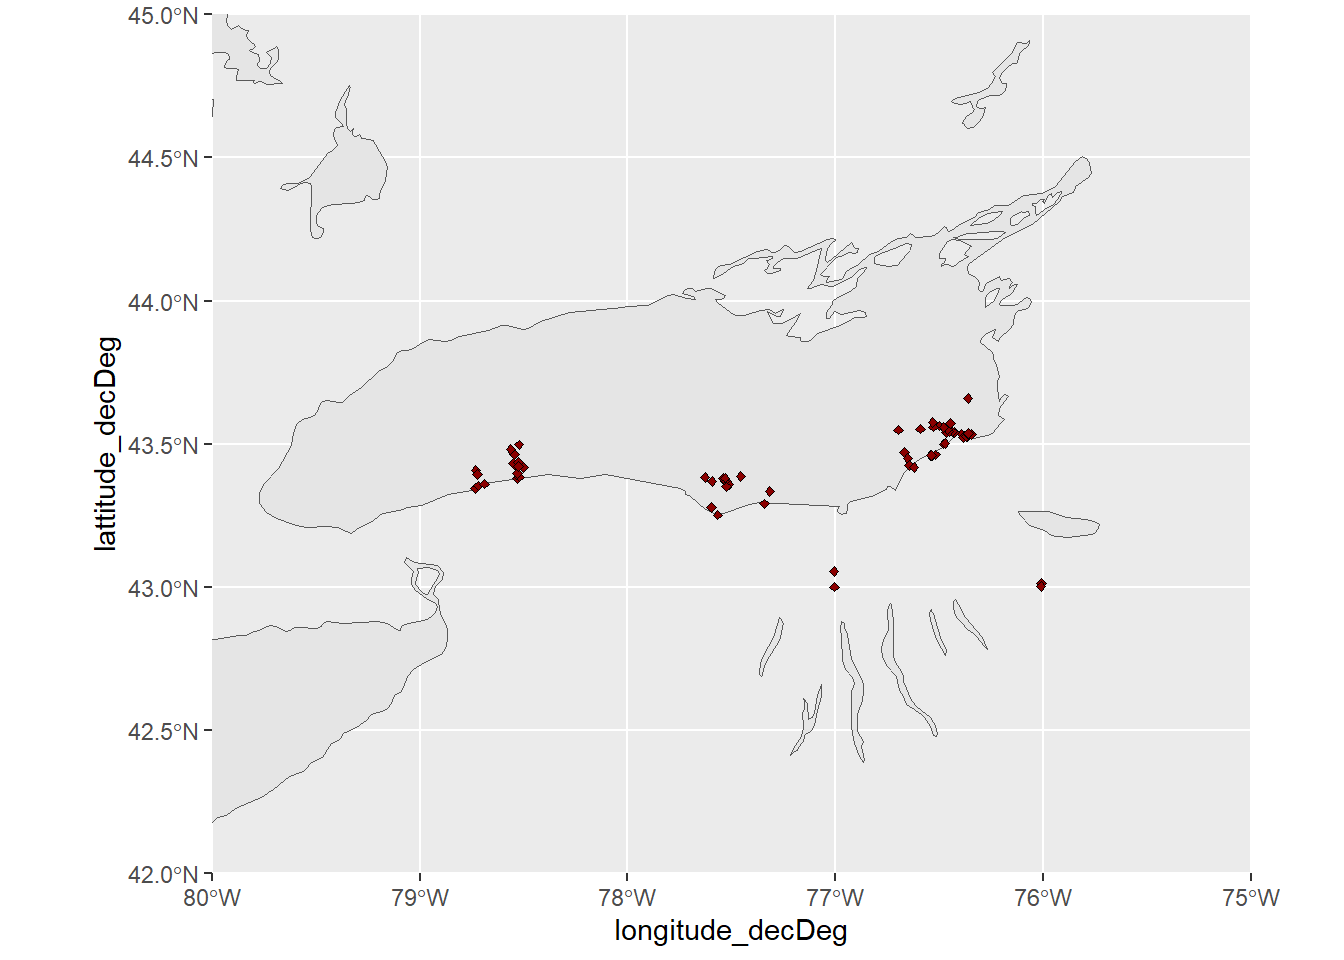
\includegraphics{ON_CSMI2013_Zoop_Data_Exploration_files/figure-latex/Create map of sample locations-1.pdf}

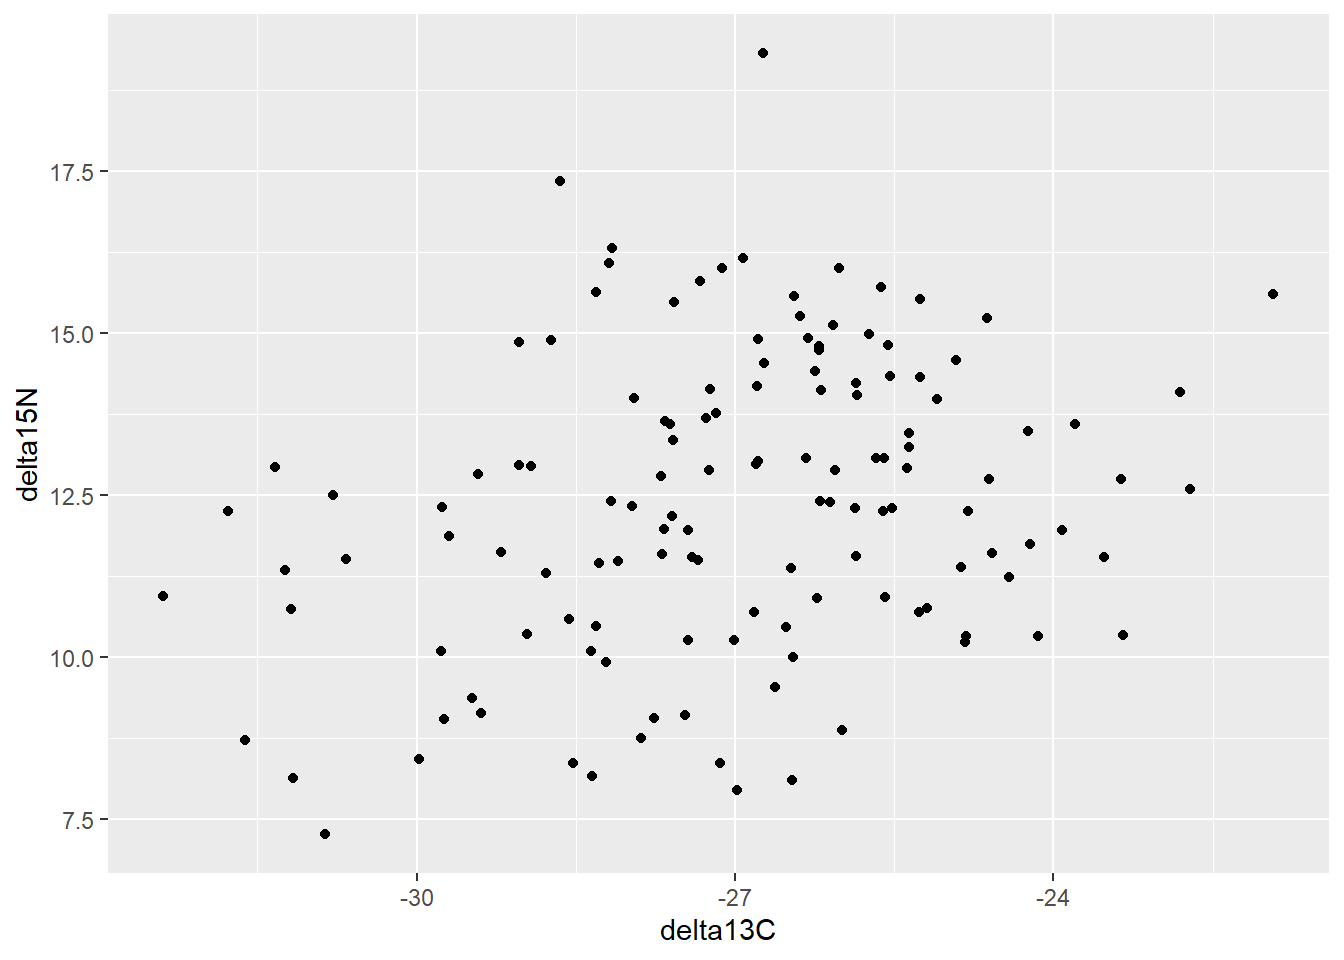
\includegraphics{ON_CSMI2013_Zoop_Data_Exploration_files/figure-latex/Start plotting-1.pdf}
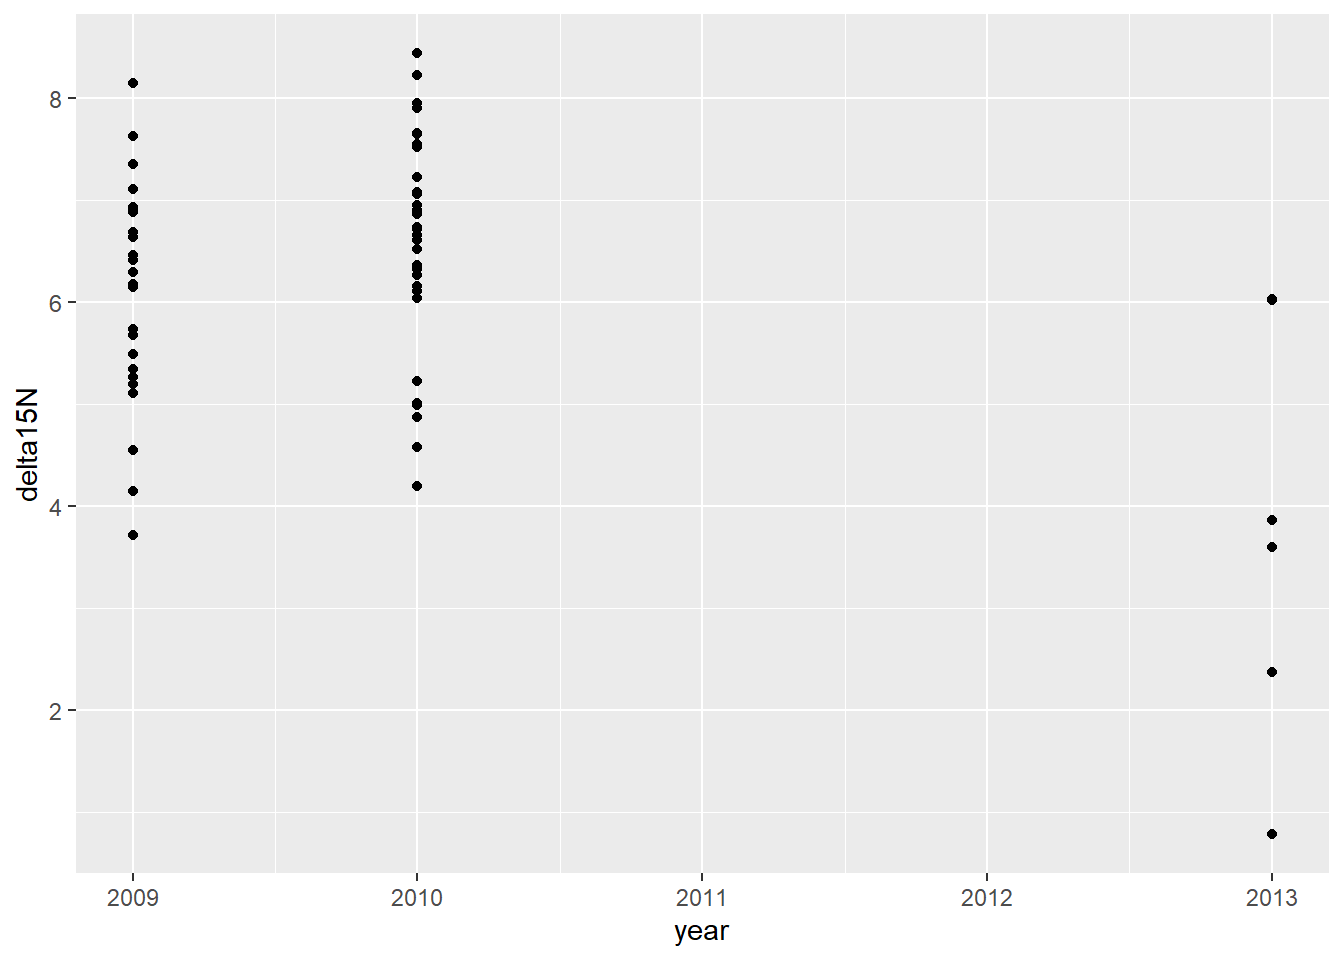
\includegraphics{ON_CSMI2013_Zoop_Data_Exploration_files/figure-latex/Start plotting-2.pdf}
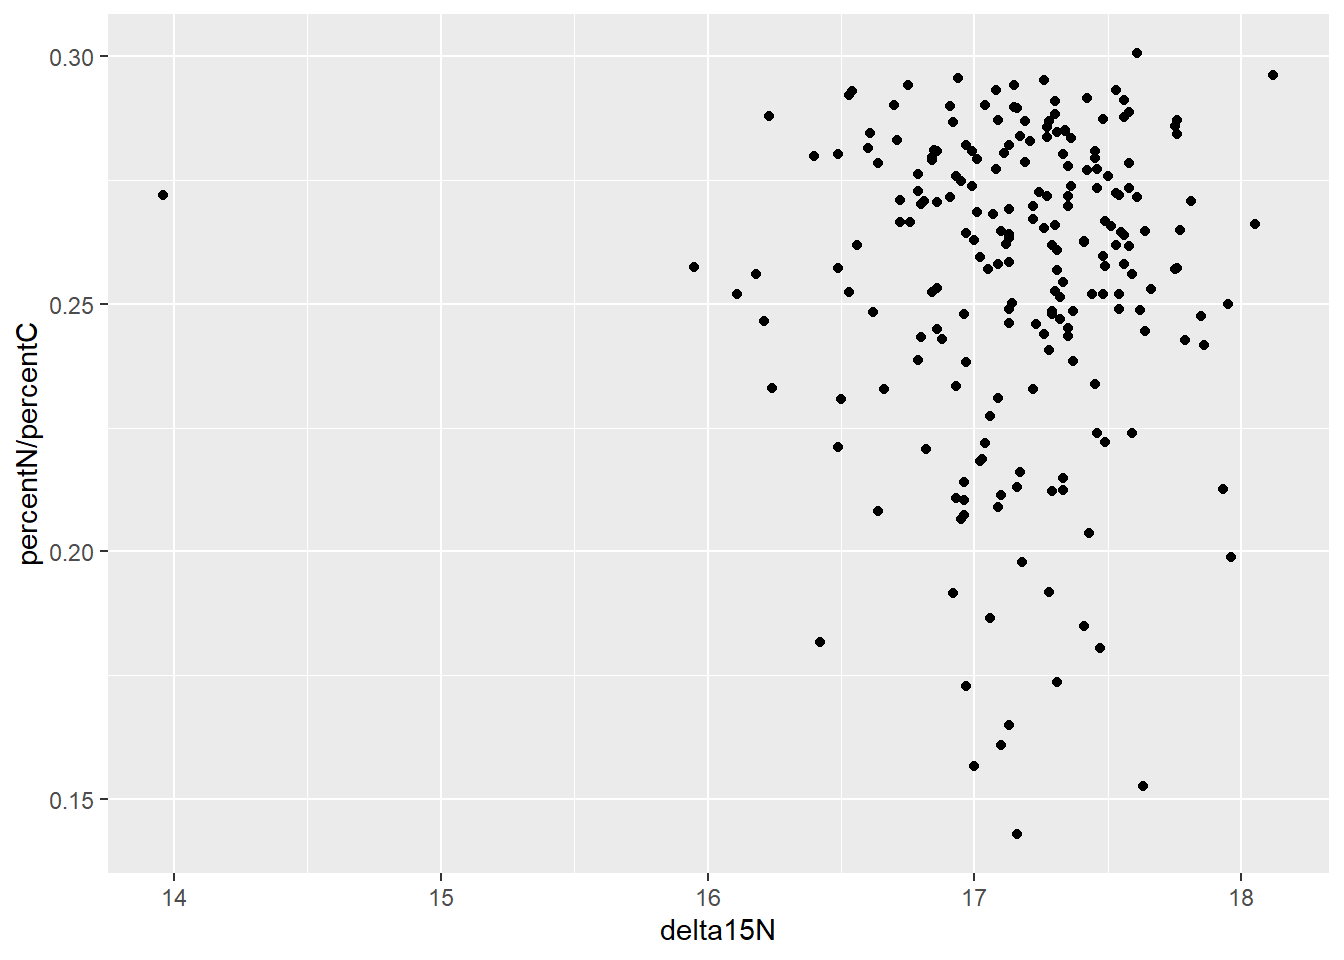
\includegraphics{ON_CSMI2013_Zoop_Data_Exploration_files/figure-latex/Start plotting-3.pdf}
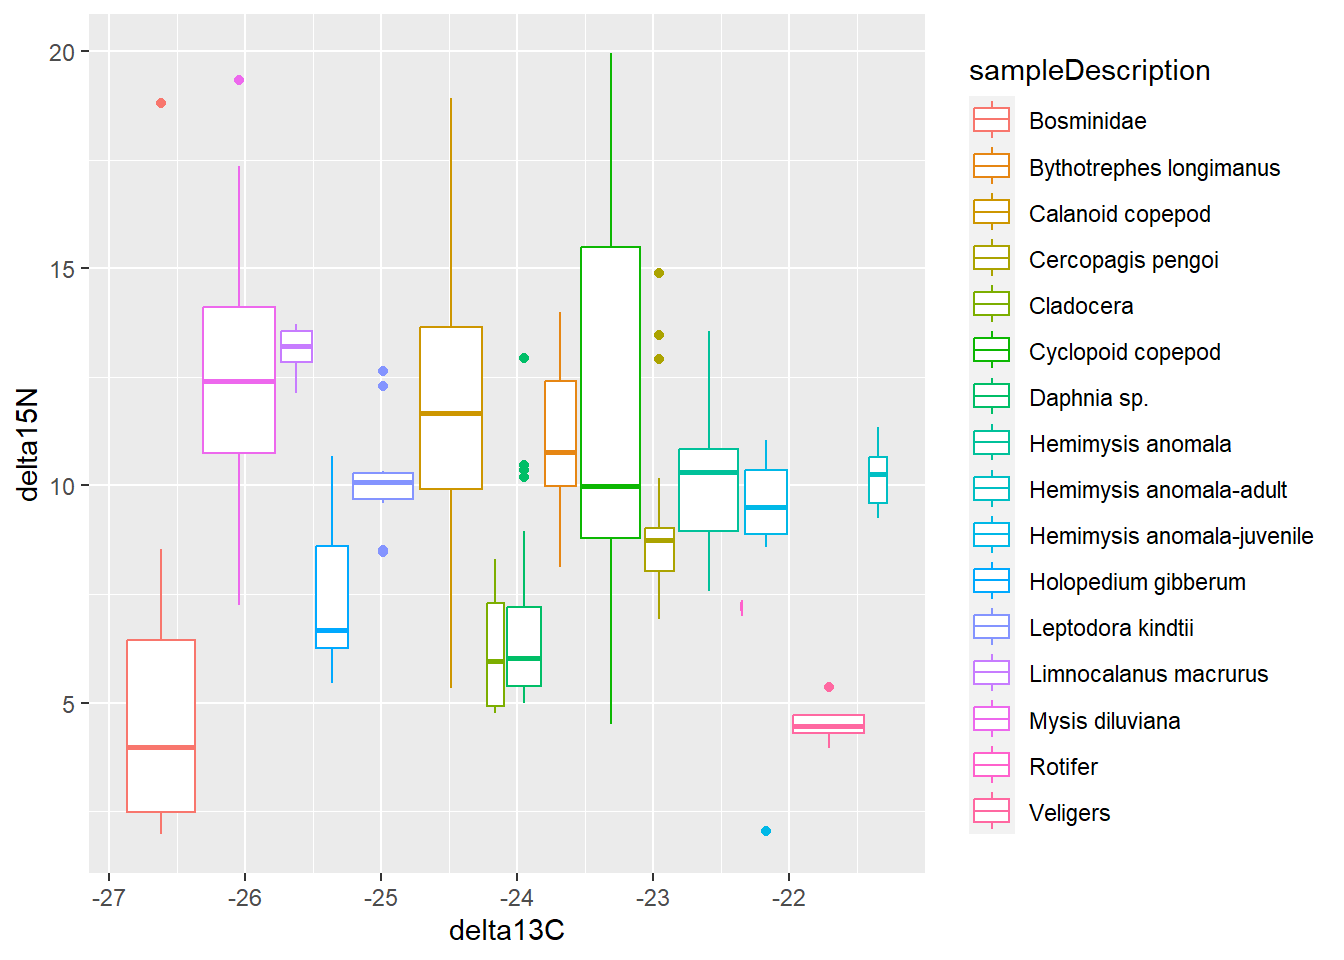
\includegraphics{ON_CSMI2013_Zoop_Data_Exploration_files/figure-latex/Start plotting-4.pdf}
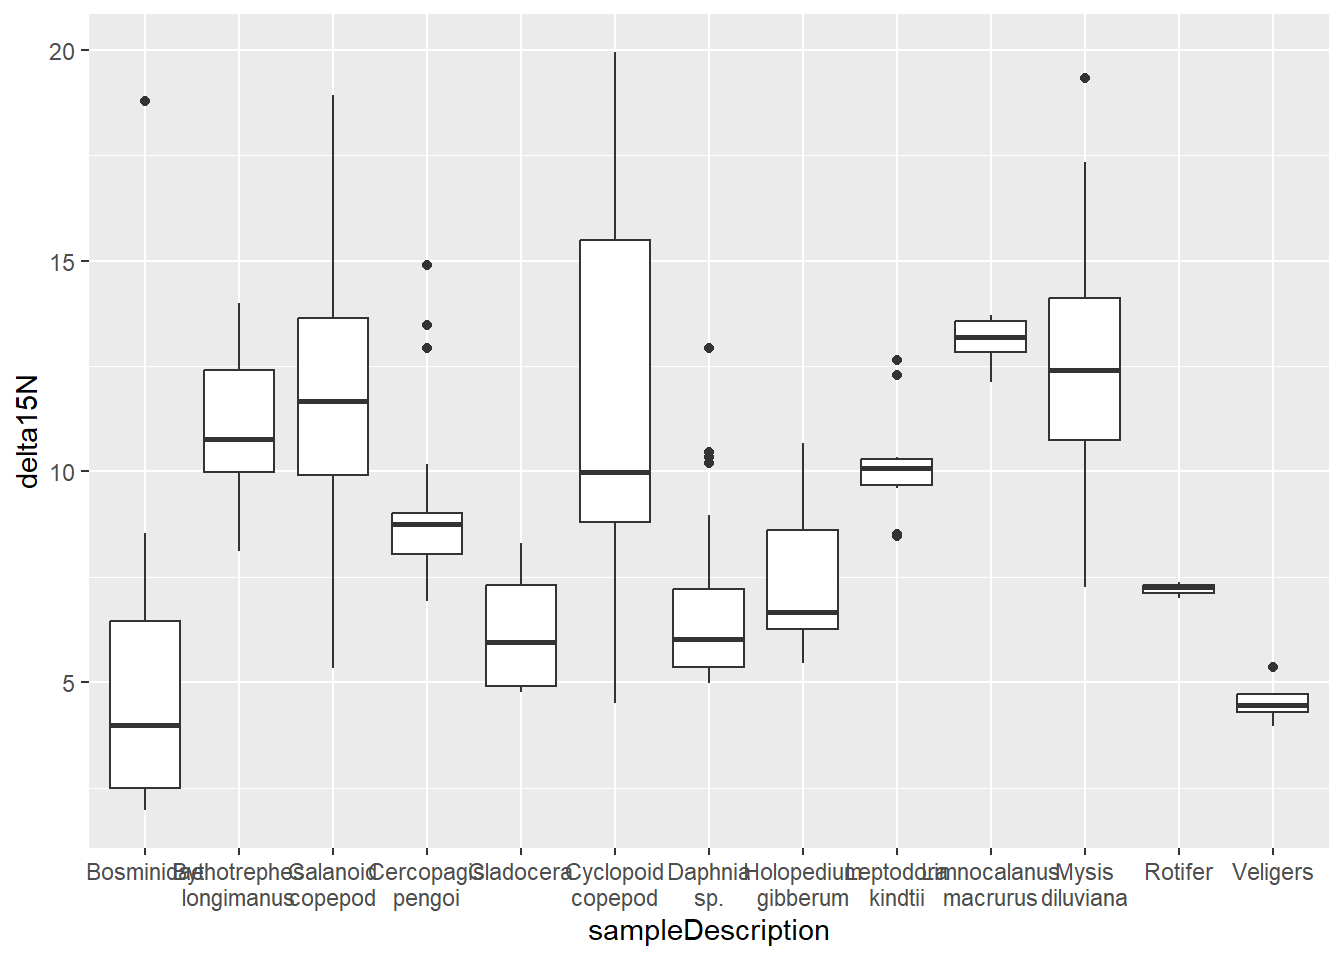
\includegraphics{ON_CSMI2013_Zoop_Data_Exploration_files/figure-latex/Start plotting-5.pdf}
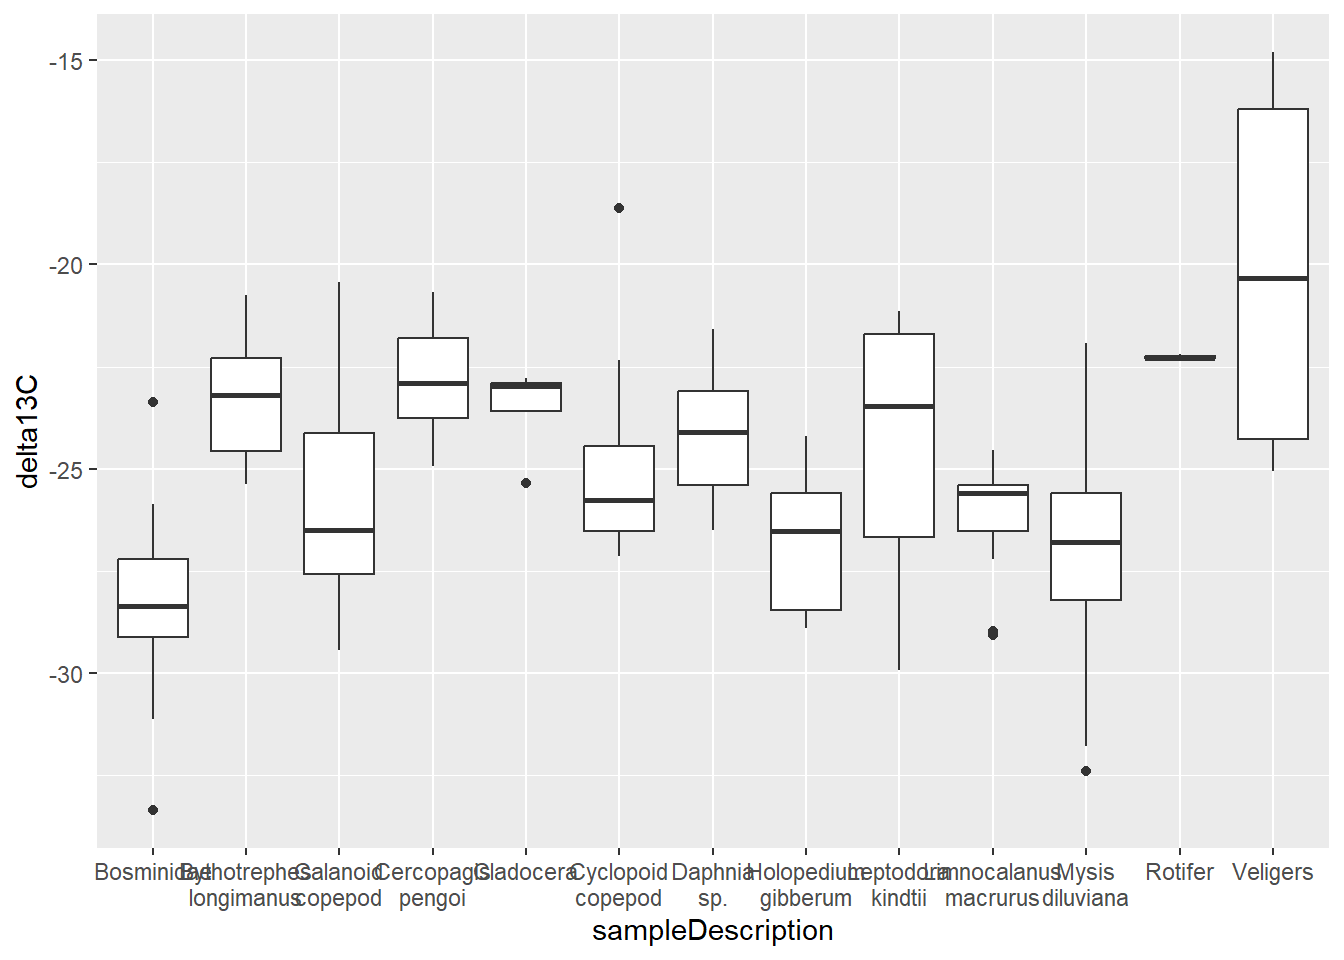
\includegraphics{ON_CSMI2013_Zoop_Data_Exploration_files/figure-latex/Start plotting-6.pdf}
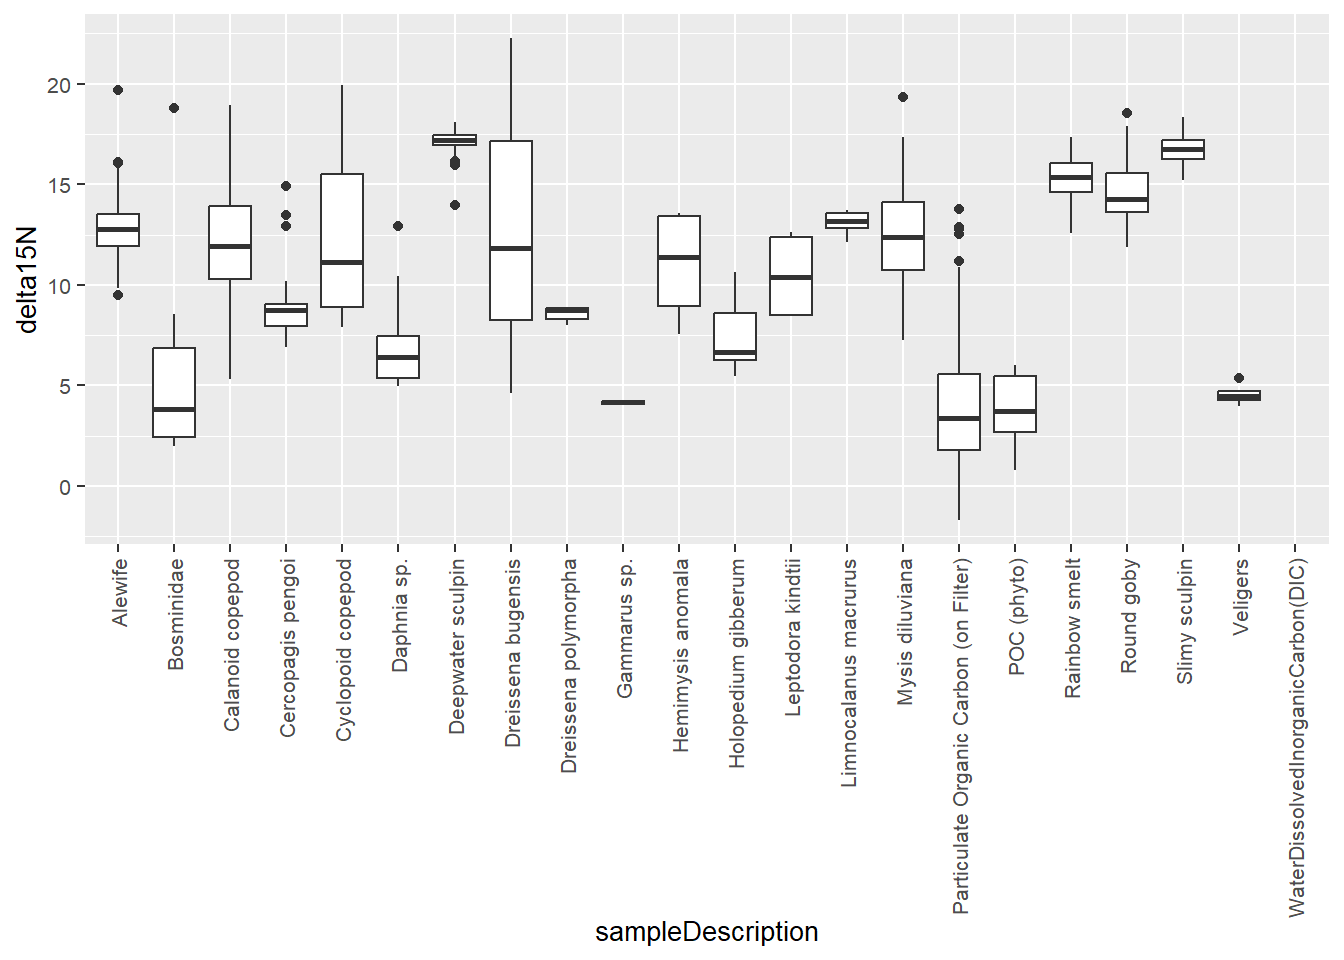
\includegraphics{ON_CSMI2013_Zoop_Data_Exploration_files/figure-latex/Start plotting-7.pdf}
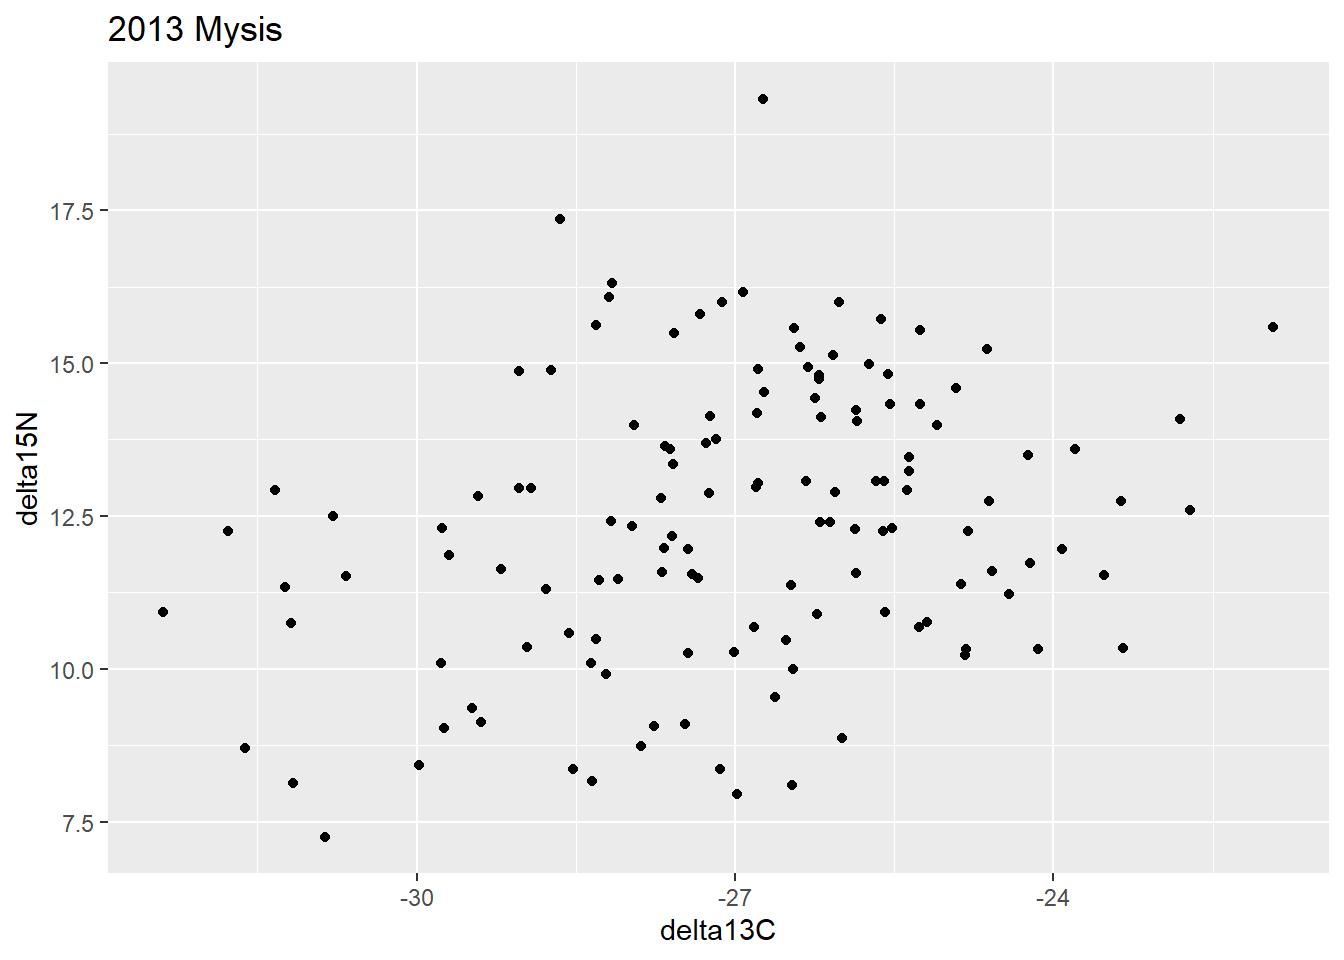
\includegraphics{ON_CSMI2013_Zoop_Data_Exploration_files/figure-latex/Start plotting-8.pdf}
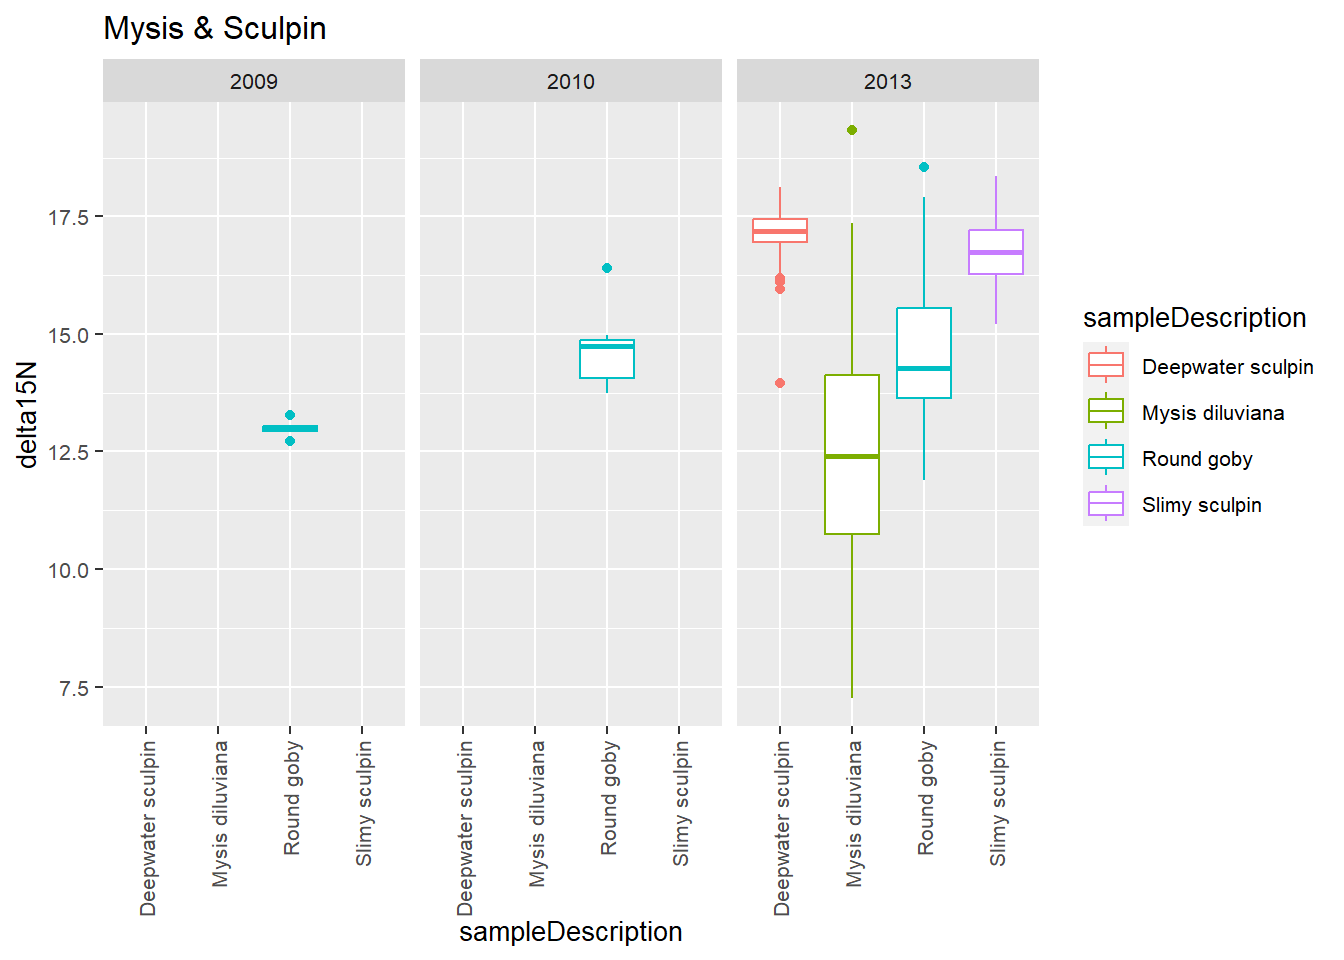
\includegraphics{ON_CSMI2013_Zoop_Data_Exploration_files/figure-latex/Start plotting-9.pdf}
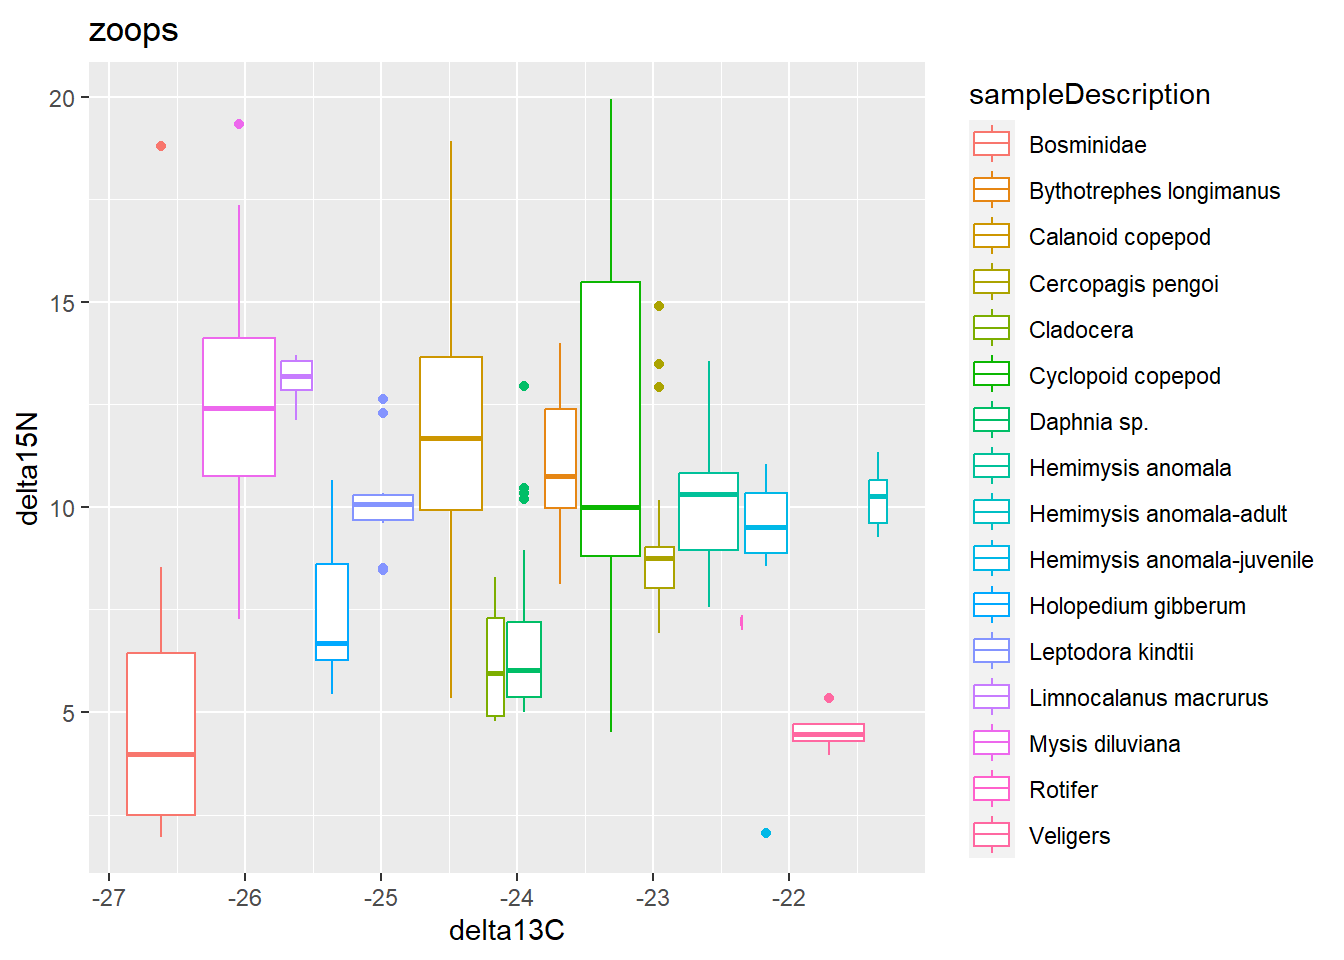
\includegraphics{ON_CSMI2013_Zoop_Data_Exploration_files/figure-latex/Start plotting-10.pdf}
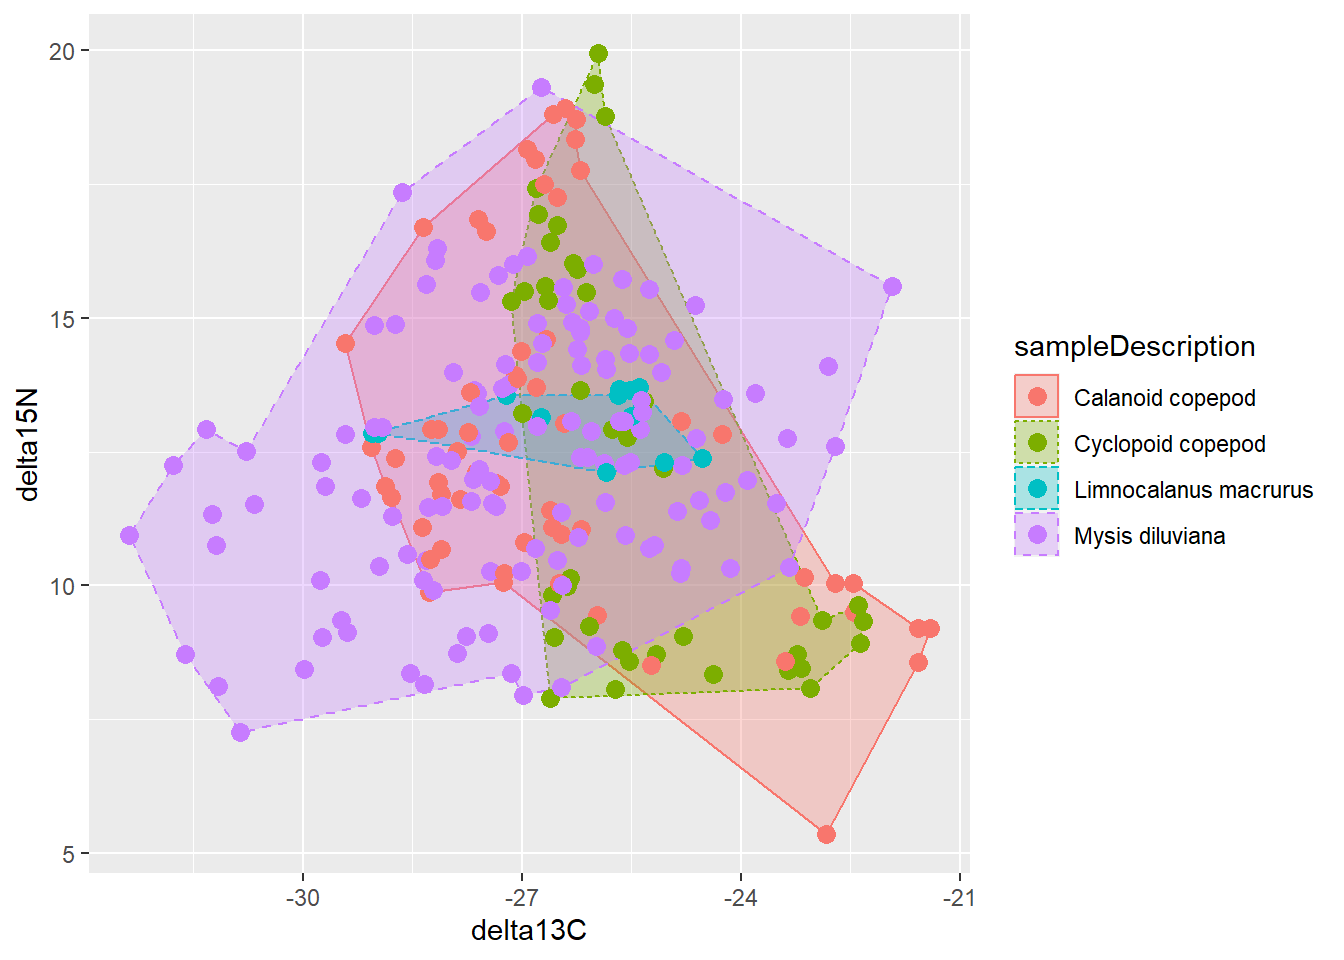
\includegraphics{ON_CSMI2013_Zoop_Data_Exploration_files/figure-latex/Start plotting-11.pdf}
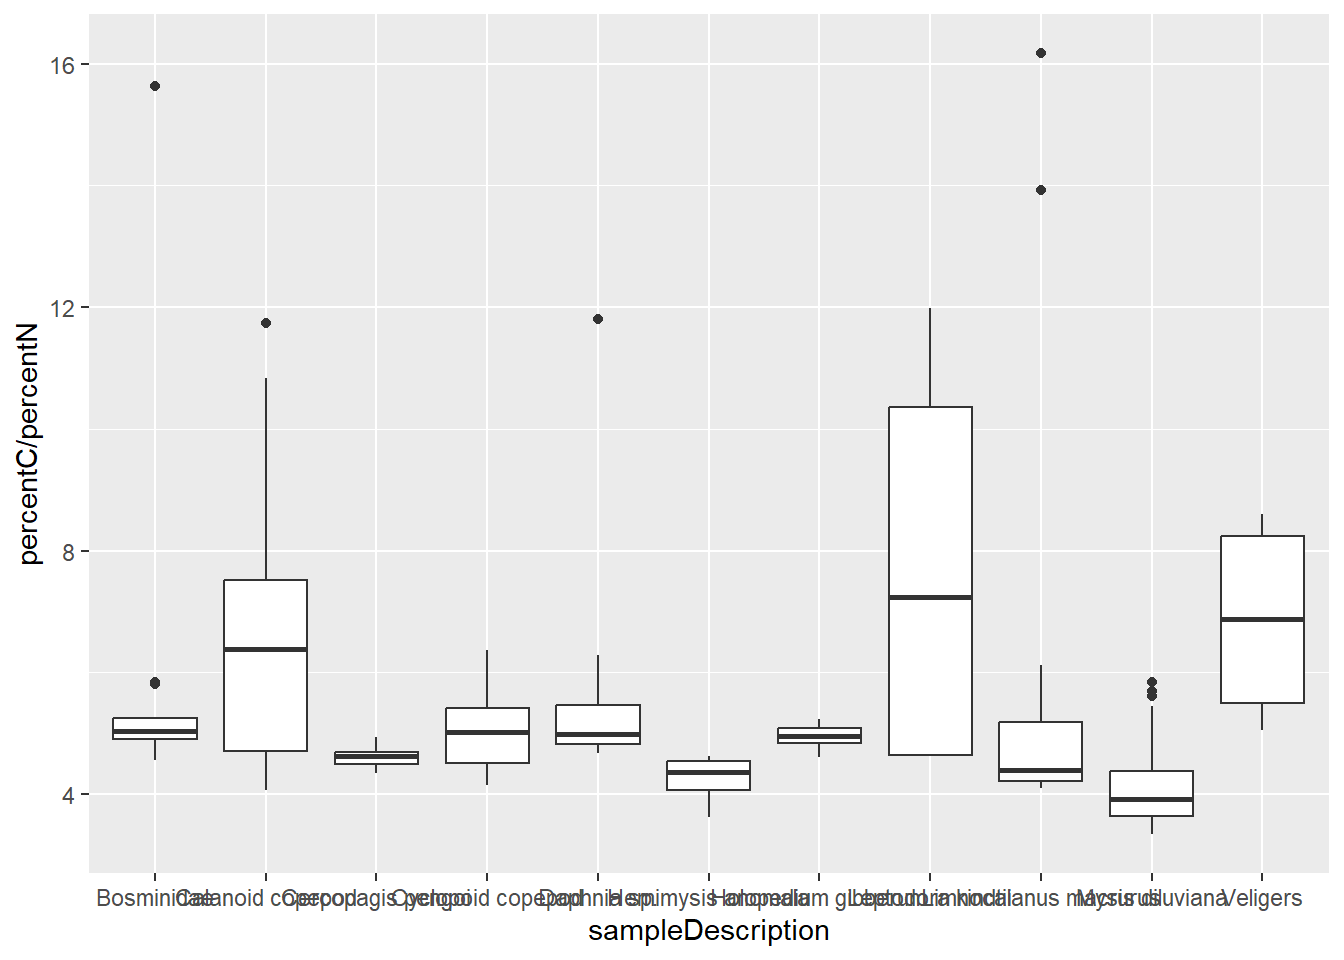
\includegraphics{ON_CSMI2013_Zoop_Data_Exploration_files/figure-latex/Start plotting-12.pdf}
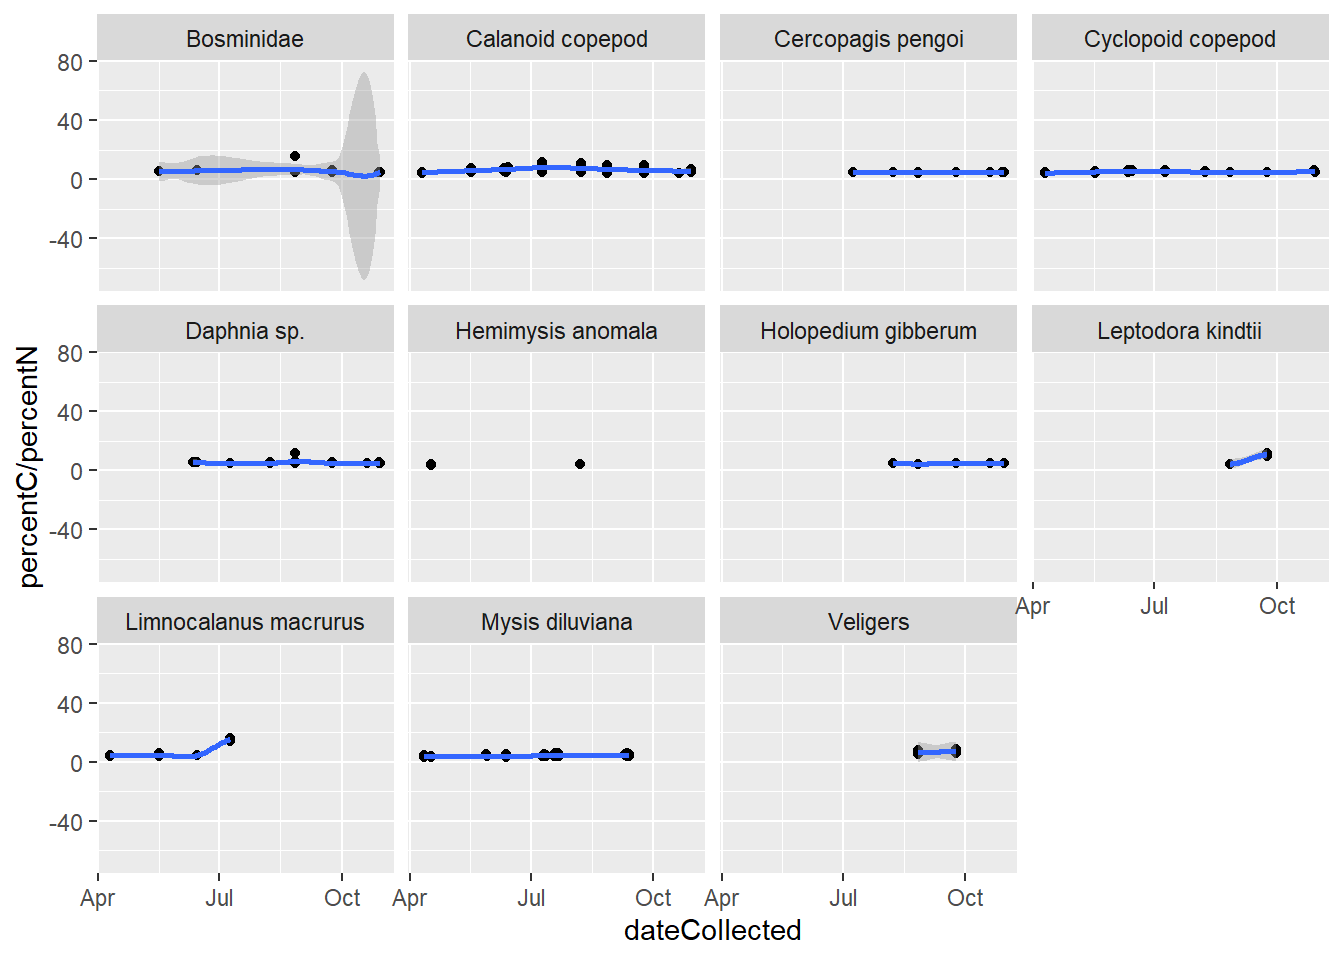
\includegraphics{ON_CSMI2013_Zoop_Data_Exploration_files/figure-latex/Start plotting-13.pdf}
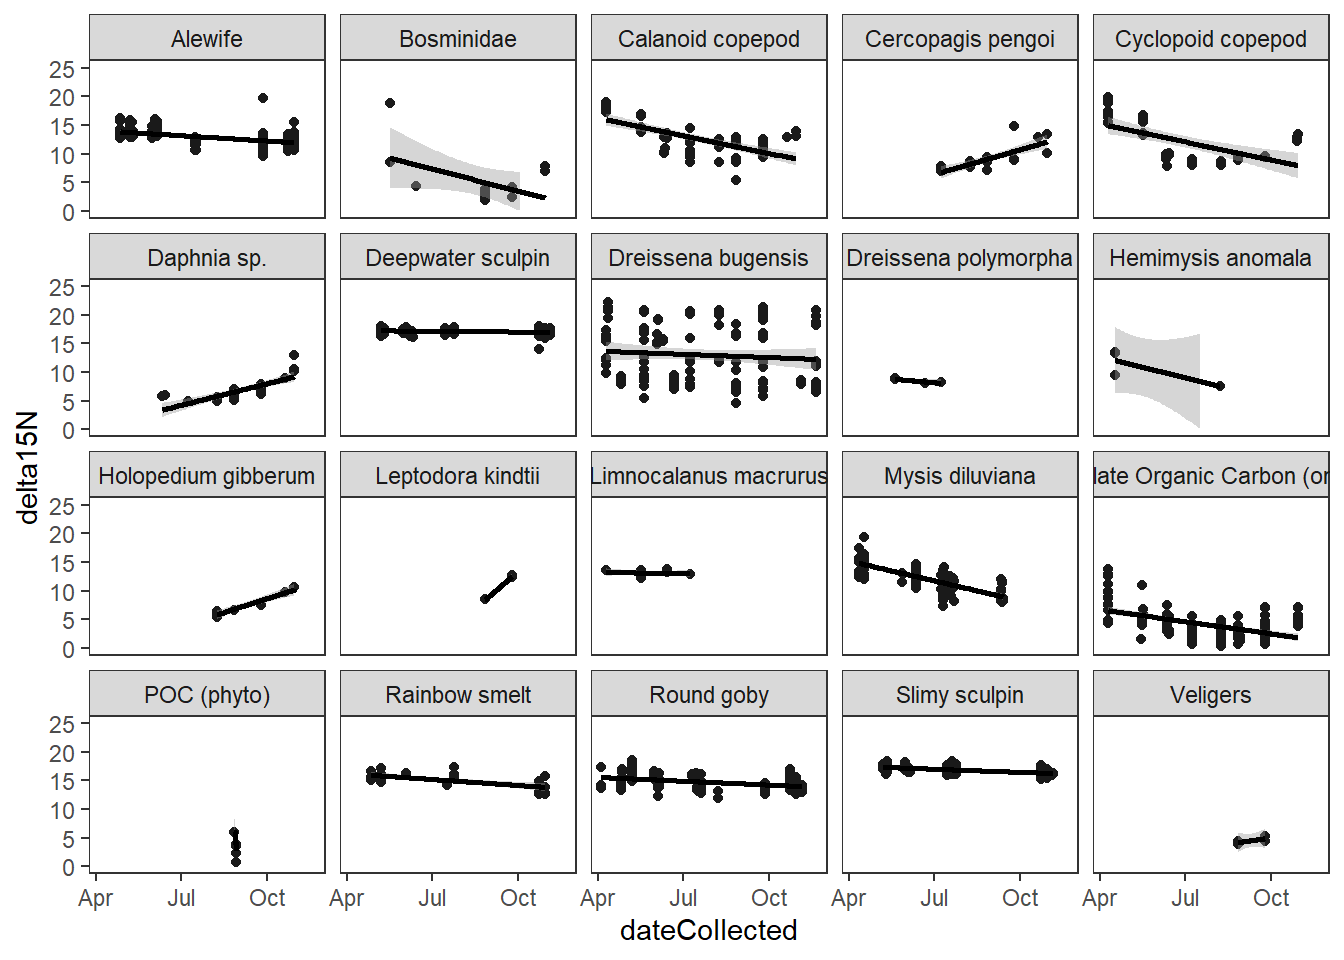
\includegraphics{ON_CSMI2013_Zoop_Data_Exploration_files/figure-latex/Start plotting-14.pdf}
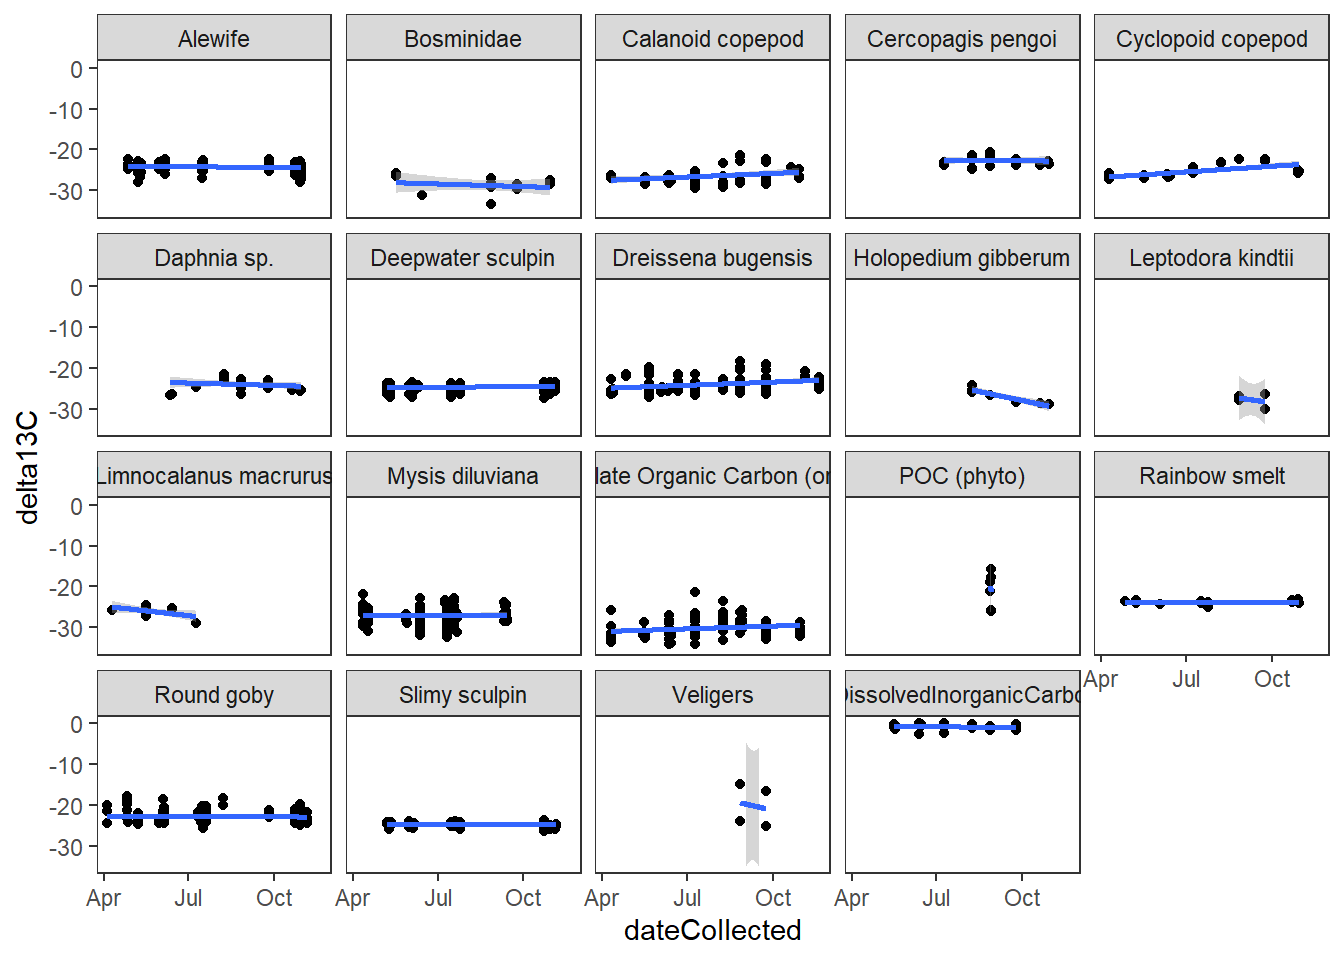
\includegraphics{ON_CSMI2013_Zoop_Data_Exploration_files/figure-latex/Start plotting-15.pdf}
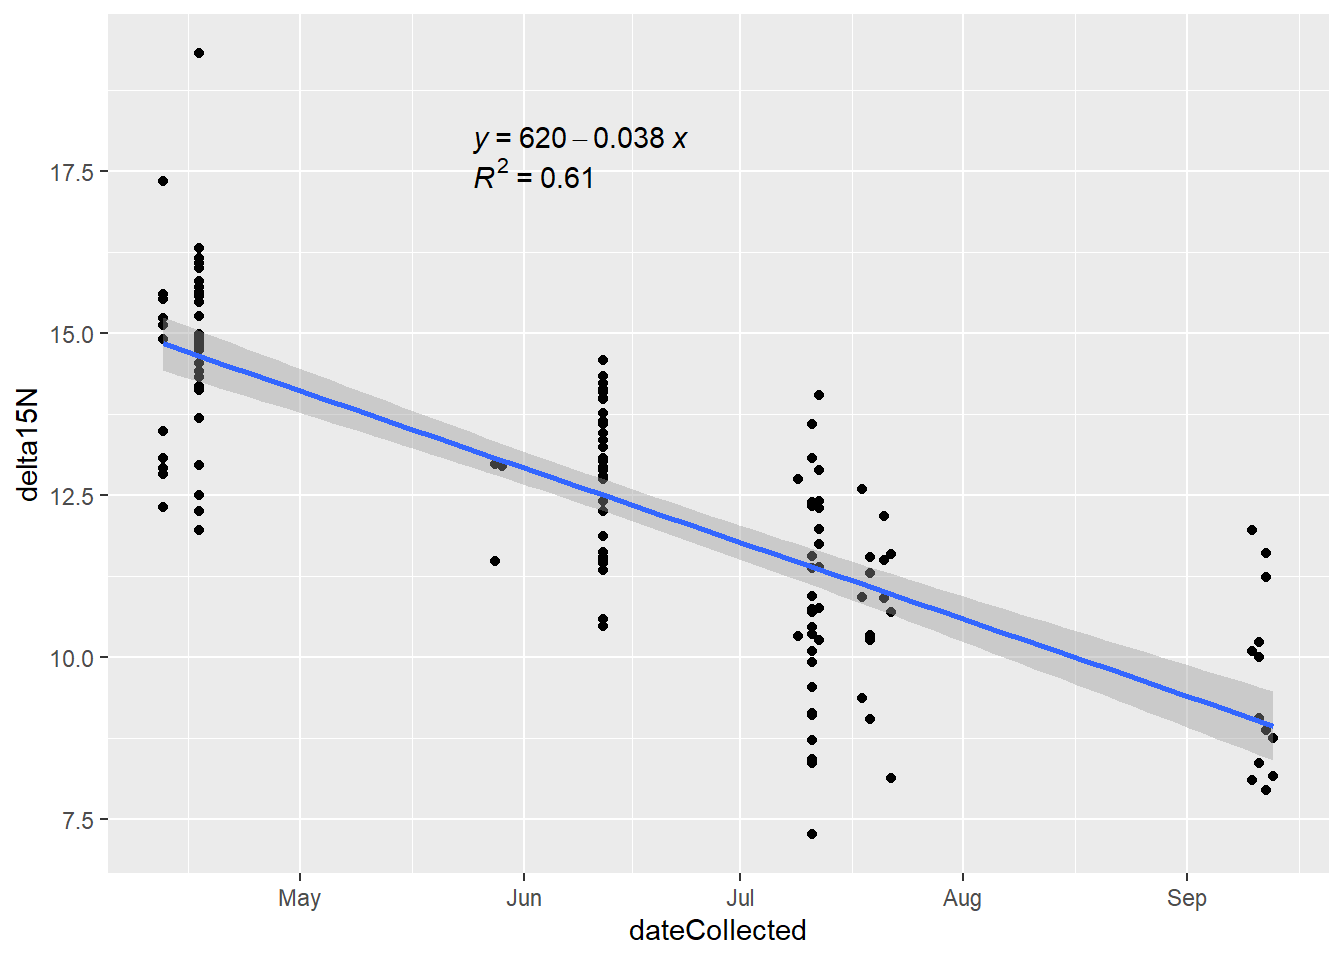
\includegraphics{ON_CSMI2013_Zoop_Data_Exploration_files/figure-latex/Start plotting-16.pdf}
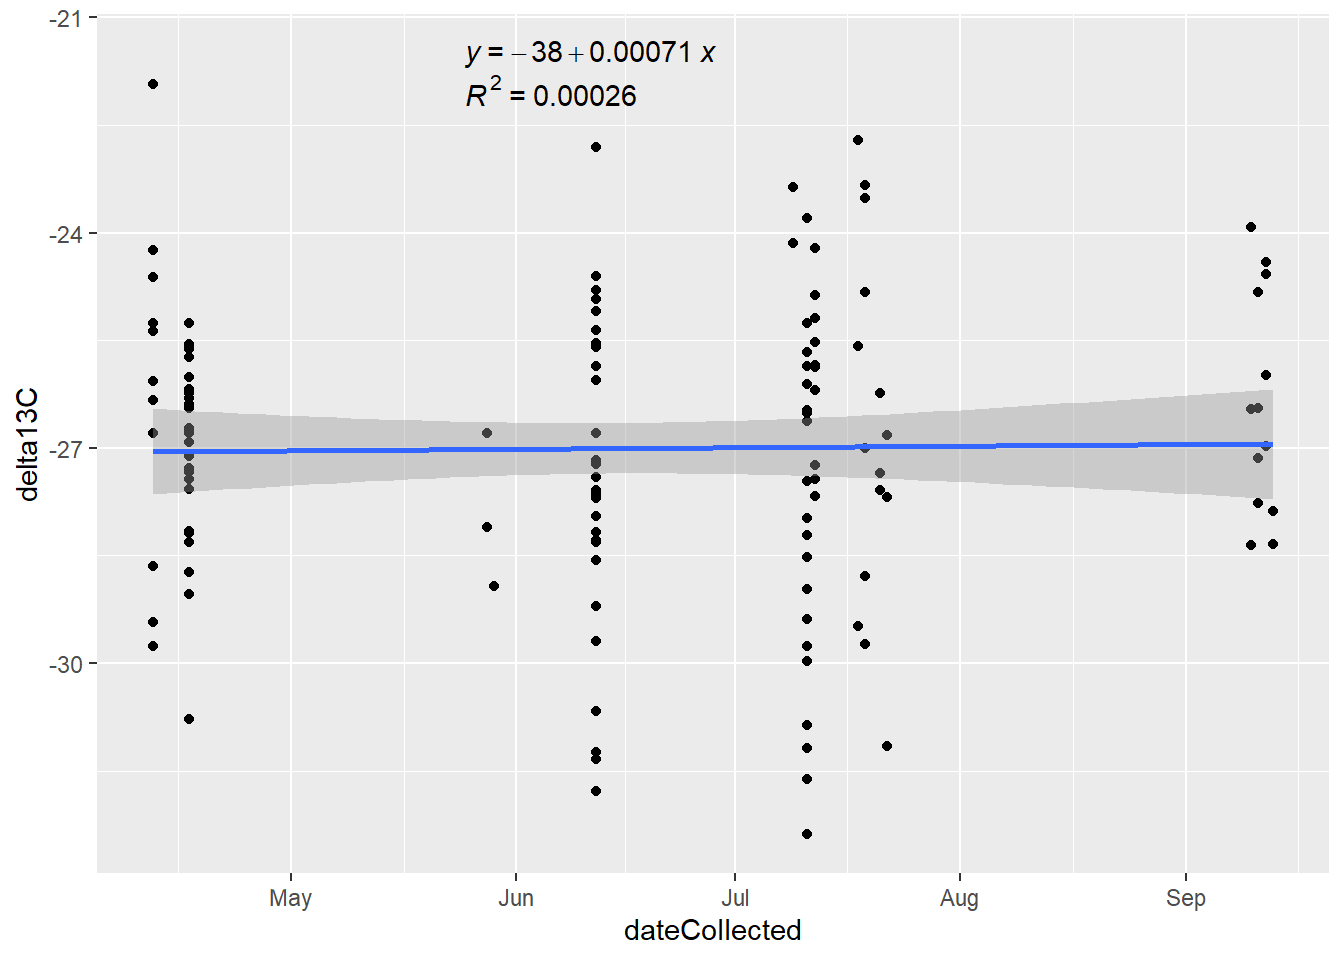
\includegraphics{ON_CSMI2013_Zoop_Data_Exploration_files/figure-latex/Start plotting-17.pdf}
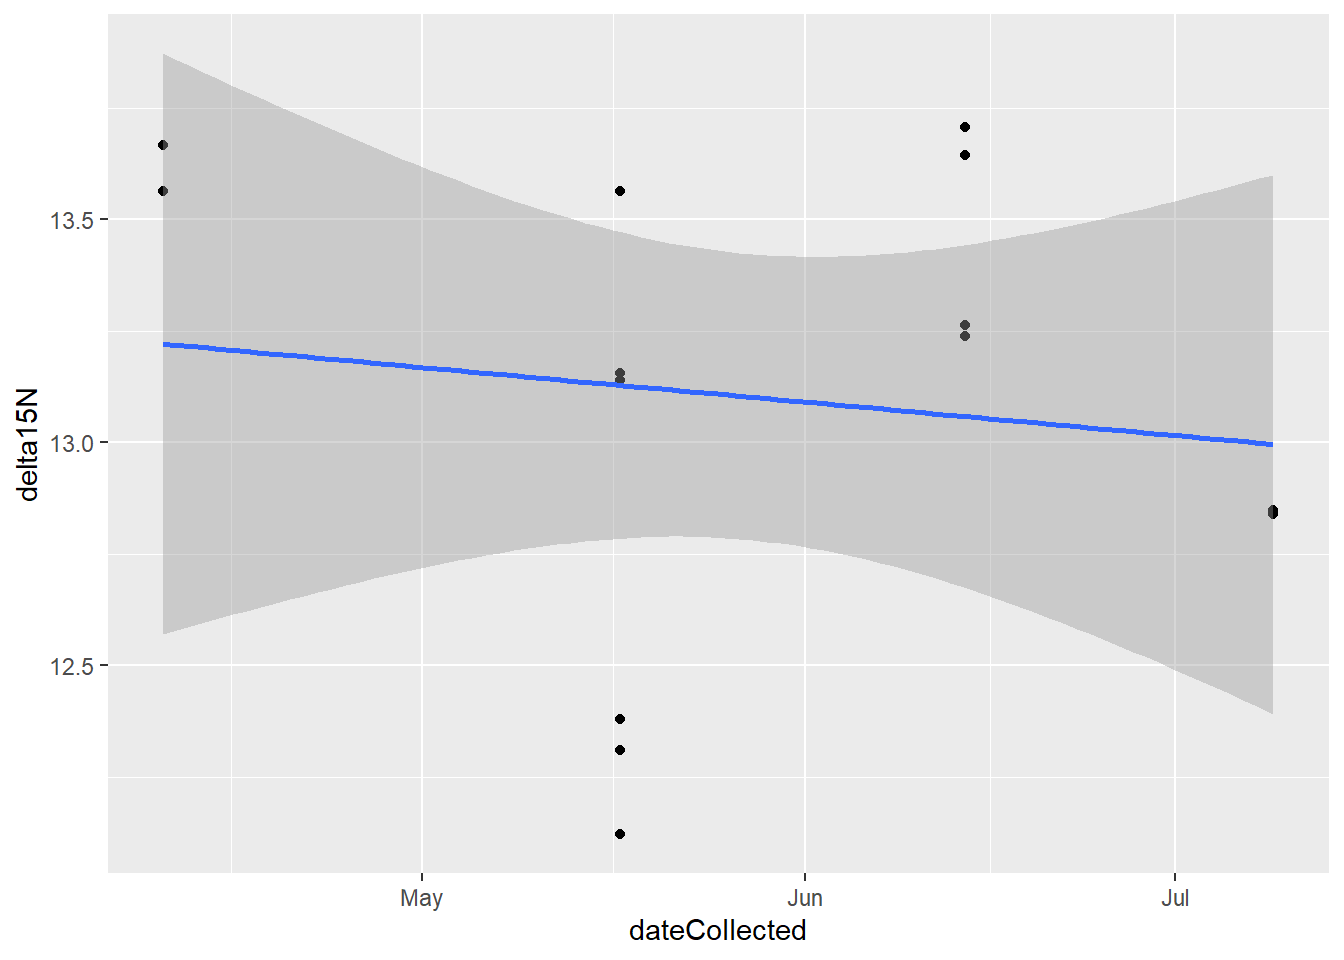
\includegraphics{ON_CSMI2013_Zoop_Data_Exploration_files/figure-latex/Start plotting-18.pdf}

\begin{verbatim}
## 
## Call:
## lm(formula = delta15N ~ dateCollected, data = mysids)
## 
## Coefficients:
##   (Intercept)  dateCollected  
##     620.71145       -0.03833
\end{verbatim}

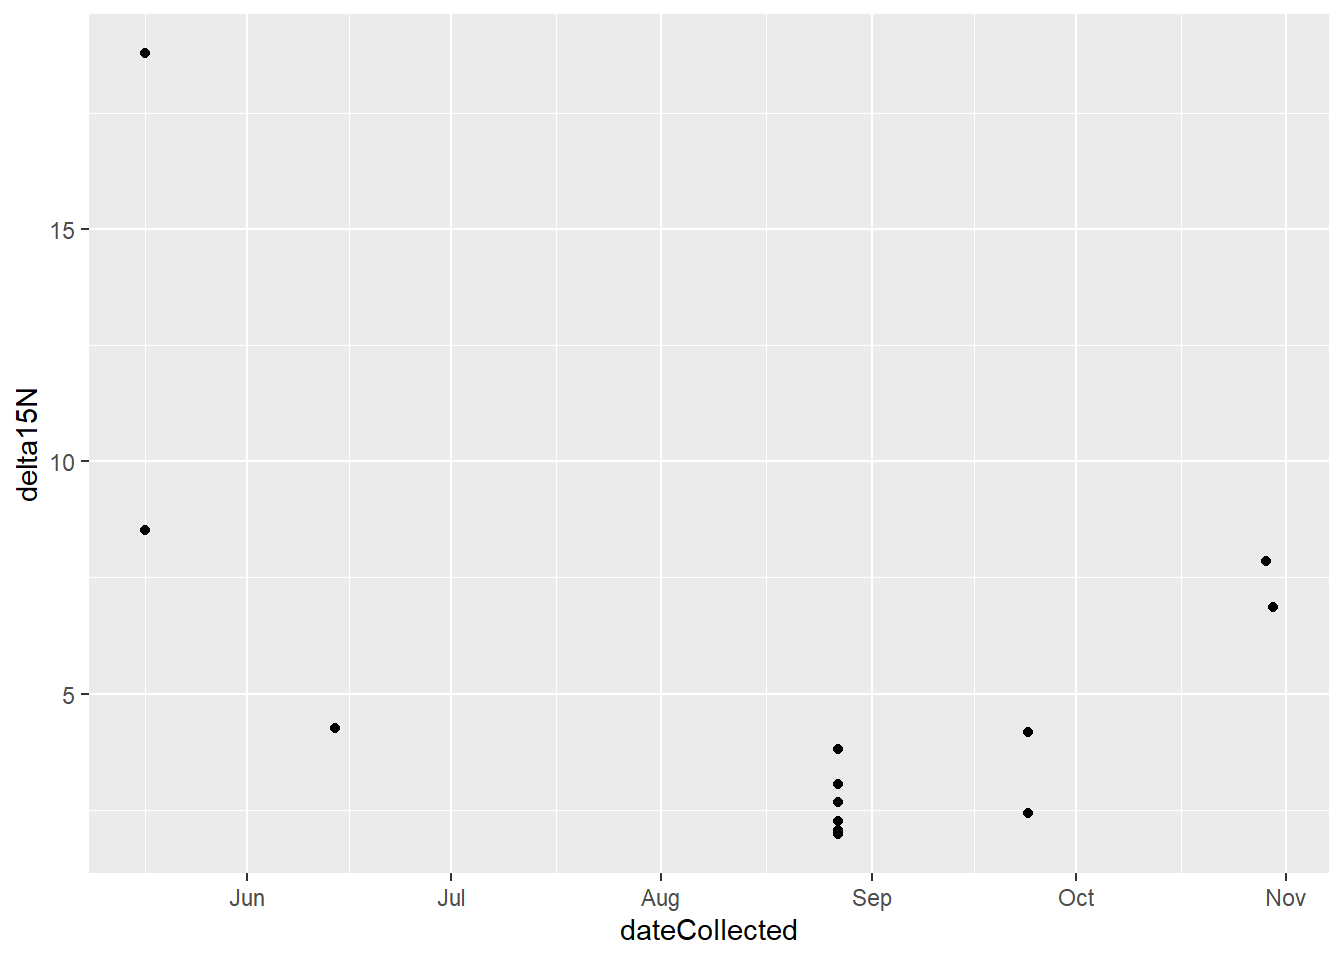
\includegraphics{ON_CSMI2013_Zoop_Data_Exploration_files/figure-latex/Start plotting-19.pdf}
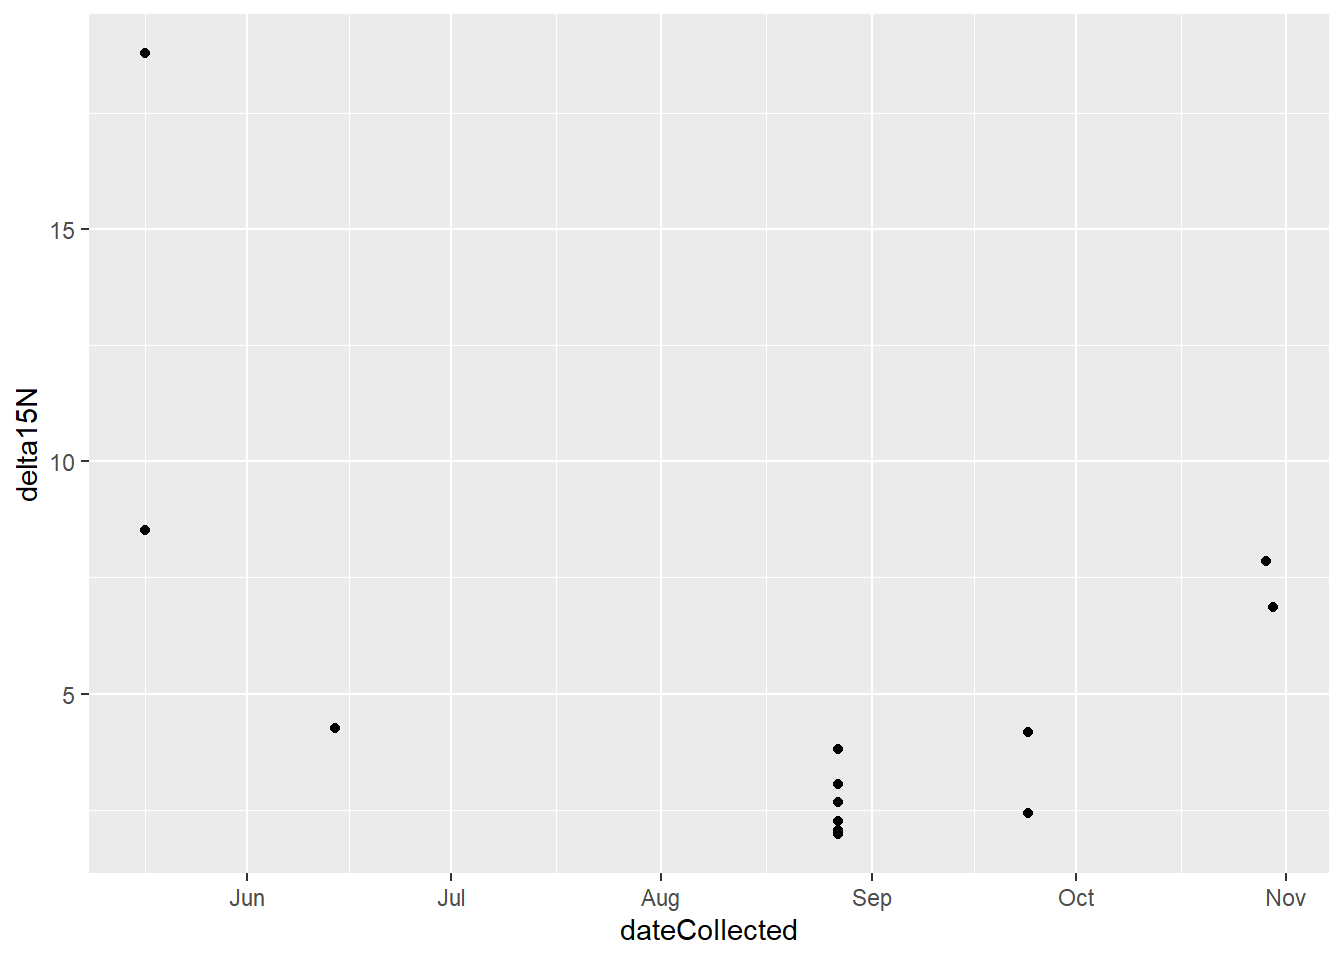
\includegraphics{ON_CSMI2013_Zoop_Data_Exploration_files/figure-latex/Start plotting-20.pdf}

\end{document}
